\documentclass[12pt, titlepage]{article}


\usepackage{amsmath, mathtools}
\usepackage{amsfonts}
\usepackage{amssymb}


\usepackage{caption}
\usepackage{pdflscape}
\usepackage{afterpage}
\usepackage{caption}
\usepackage{pbox}
\usepackage{makecell}


\usepackage{booktabs}
\usepackage{tabularx}
\usepackage{hyperref}
\hypersetup{
    colorlinks,
    citecolor=black,
    filecolor=black,
    linkcolor=red,
    urlcolor=blue
}
\usepackage[sort&compress,square,comma,numbers]{natbib}
\newcounter{reqnum} %Requirement Number
\newcommand{\myprogname}{Lattice Boltzmann Solver} 

%% Comments

\usepackage{color}

\newif\ifcomments\commentstrue

\ifcomments
\newcommand{\authornote}[3]{\textcolor{#1}{[#3 ---#2]}}
\newcommand{\todo}[1]{\textcolor{red}{[TODO: #1]}}
\else
\newcommand{\authornote}[3]{}
\newcommand{\todo}[1]{}
\fi

\newcommand{\wss}[1]{\authornote{blue}{SS}{#1}} 
\newcommand{\plt}[1]{\authornote{magenta}{TPLT}{#1}} %For explanation of the template
\newcommand{\an}[1]{\authornote{cyan}{Author}{#1}}

%% Common Parts

\newcommand{\progname}{ProgName} % PUT YOUR PROGRAM NAME HERE %Every program
                                % should have a name


\begin{document}


\title{System Verification and Validation Plan for \myprogname} 
\author{Peter Michalski}
\date{\today}
	
\maketitle

\pagenumbering{roman}

\section{Revision History}

\begin{tabularx}{\textwidth}{p{4cm}p{2cm}X}
\toprule {\bf Date} & {\bf Version} & {\bf Notes}\\
\midrule
October 28, 2019 & 1.0 & Initial Document\\
\bottomrule
\end{tabularx}

\newpage

\tableofcontents

\newpage

\listoftables

\listoffigures

\newpage

\section{Symbols, Abbreviations and Acronyms}

\subsection{Abbreviations and Acronyms}
\renewcommand{\arraystretch}{1.2}
\begin{tabular}{l l} 
  \toprule		
  \textbf{symbol} & \textbf{description}\\
  \midrule 
  1D & One Dimensional\\
  2D & Two Dimensional\\
  A & Assumption\\
  C & Pseudo-Oracle Control Value\\
  CA & Commonality Analysis\\
  V & All Input Values\\
  I & Individual Parameter Input Values\\
  IDE & Integrated Development Environment\\
  LBM & Lattice Boltzmann Method\\
  LBS & Lattice Boltzmann Solvers\\
  MG & Module Guide\\
  MIS & Module Interface Specification\\
  MTBF & Mean Time Between Failures\\
  NAN & Not A Number\\
  NFR & Non-Functional Requirement\\
  O & Program Output\\
  OTS & Off The Shelf\\
  P & Program\\
  R & Functional Requirement\\
  SRS & Software Requirement Specification\\
  VnV & Verification and Validation\\
  \bottomrule
\end{tabular}\\

\newpage

\subsection{Symbols}

\renewcommand{\arraystretch}{1.2}
\begin{tabular}{l l} 
  \toprule		
  \textbf{symbol} & \textbf{description}\\
  \midrule 
  $Re$ & Reynolds Number\\
  $\rho$ & Density \\
  $t$ & Time \\
  $\eta_b$ & Bulk Viscosity \\
  $\eta_s$ & Shear Viscosity \\
  $\mathbb{N}$ & natural numbers\\
  $X_{min}$ & Lowest X-Axis Interval of Boundary\\
  $X_{max}$ & Highest X-Axis Interval of Boundary\\
  $Y_{min}$ & Lowest Y-Axis Interval of Boundary\\
  $Y_{max}$ & Highest Y-Axis Interval of Boundary\\
  $R$ & Radius of Cylinder\\
  $\mathrm{e_{sch}}$ & Velocity Slowdown Factor\\
  $\mathrm{e_{fac}}$ & Velocity of Scheme\\
  $S$ & Spatial Step - Number of Spatial Subsections\\
  $\mathrm{e_{max}}$ & Max Velocity in the Middle of Channel\\
  $\mathrm{D}$ & Signifies the Dimension Component of Lattice Model\\
  $\mathrm{Q}$ & Signifies Number of Velocity Directions of Lattice Model\\
  $D_{l}$ & Length of the Domain\\
  $D_{w}$ & Width of the Domain\\
  $E_r$ & Relative Error\\
  \bottomrule
\end{tabular}\\

\newpage

\pagenumbering{arabic}

\noindent This document covers the system Verification and Validation (VnV) of \myprogname . Functional and non-functional requirements, as found in Section \ref{objectives} and retrieved from the Commonality Analysis (CA) (\citet{LBM_CA_PM}), will be tested. The document will outline the general information of the system in Section \ref{generalinfo}, which will be followed by a testing plan in Section \ref{testplan}. Finally, individual tests will be described in Section \ref{systest}. 

\section{General Information}
\label{generalinfo}
\subsection{Summary}

The software being tested is \myprogname . This software reads inputs from a file, and calculates outputs using Lattice Boltzmann Methods (LBM).The software outputs the results to the screen, to a file, and/or to memory.\\ 

\noindent {\myprogname} can model many fluid dynamics problems, including Poiseuille Flow and Von Karman Vortex Street. Both of these problems will be used in our functional test cases, as the results of {\myprogname} can be compared to the results of the pseudo-oracle pyLBM (\citet{pylbmcode}).

\subsection{Objectives}
\label{objectives}

The intended objective of this plan is to verify that functional requirements and non-functional requirements (NFR), as found in the CA titled Lattice Boltzmann Solvers (\citet{LBM_CA_PM}), have been met.\\ 

\noindent The functional requirements are:\\
\noindent \begin{itemize}
\item[R\refstepcounter{reqnum}\thereqnum \label{R_Inputs}:] The system shall read a set of input fluid parameters.

\item[R\refstepcounter{reqnum}\thereqnum \label{R_ModelInputs}:] The system shall allow the user to select from a set of model and velocity direction parameters.

\item[R\refstepcounter{reqnum}\thereqnum \label{R_CheckInputs}:] The system shall verify that the inputs fall within the allowable parameters of variation.

\item[R\refstepcounter{reqnum}\thereqnum \label{R_Instantiate}:] The system shall instantiate required data types and structures for the selected model.

\item[R\refstepcounter{reqnum}\thereqnum \label{R_CoefficientWeights}:] The system shall import the relevant coefficient weights for the selected model.

\item[R\refstepcounter{reqnum}\thereqnum \label{R_Calculate}:] The system shall calculate and store the predicted fluid parameters, iterating through streaming and collision processes over the desired model time.

\item[R\refstepcounter{reqnum}\thereqnum \label{R_Output}:] The system shall output the results of the calculations in a manner consistent with the decisions made regarding variabilities.\\

\end{itemize}

\noindent The NFRs are:

\begin{enumerate}
\item Correctness: The allowable error of the output results, per module, will be less than the average error taken from the results of a sample of OTS solutions.
\item Maintainability: The system shall be documented with a CA, VnV plan, MG (Module Guide), MIS (Module Interface Specification), and User Guide.
\item Performance: The system shall be able to run modules faster than an OTS implementation.
\item Portability: The system shall be able to run on macOS, Windows, and Linux operating systems.
\item Reliability: The mean time between failures (MTBF) will be longer than the average MTBF of a sample of the OTS solutions.
\item Reusability: Individual modules of the system can be removed and reused in other systems.
\item Robustness: The system shall behave reasonably in circumstances that were not anticipated in the requirements specification \cite{ghezzi1991fundamentals}.
\item Scalability: The system must be able to support additional computational models.
\item Understandability: New users must easily understand which LBM models are available in {\myprogname}.
\item Usability: Users will find the system easy to use.
\end{enumerate}


\subsection{Relevant Documentation}

The CA of {\myprogname} can be found in (\citet{LBM_CA_PM}).\\ 

\newpage

\section{Plan}
\label{testplan}	
\subsection{Verification and Validation Team}

This VnV plan will be conducted by Peter Michalski and several classmates.

\subsection{CA Verification Plan}

The CA of {\myprogname} shall be verified in the following ways:

\begin{enumerate}
\item Feedback: Reviewers from the class shall provide feedback on GitHub.
\item Initial Review: The document shall be manually reviewed by the author using the SRS checklist upon its initial creation, as found in the CAS741 GitLab repository (\citet{CAS741_SRS_checklist}).
\item Second Review: The document shall be manually reviewed by the author using the SRS checklist after VnV completion, as found in the CAS741 GitLab repository (\citet{CAS741_SRS_checklist}).
\item Final Review: The document shall be manually reviewed by the author using the SRS checklist after MG and MIS development, as found in the CAS741 repository (\citet{CAS741_SRS_checklist}).
\end{enumerate}

\subsection{Design Verification Plan}

The design shall be verified by ensuring that functional requirements and NFRs are tested, as listed in Section \ref{objectives}.\\

\noindent The system functional requirements shall be tested first, as outlined in \ref{testfr}. This will be followed by reviewing the NFRs as outlined in \ref{nfrtest}.


\subsection{Implementation Verification Plan}
  
\noindent The implementation shall be verified in the following ways:

\begin{enumerate}
\item Code Walkthrough - Author: Module unit code shall be inspected for functional errors by the author immediately after MS document version 1.0 is developed. A rubber duck debugging method will be followed. Any defects shall be immediately fixed. This plan is described in Section 5.1 of the document Unit Verification and Validation Plan for Lattice Boltzmann Solver (\citet{LBM_UVNV_PM}).
\item Code Walkthrough - Peer: Module unit code shall be inspected for functional errors by Ao Dong after MS document version 1.0 is submitted on GitHub. Defects shall be noted in GitHub using issue creation. This plan is described in Section 5.1 of the document Unit Verification and Validation Plan for Lattice Boltzmann Solver (\citet{LBM_UVNV_PM}).
\item Dynamic Unit Tests - Author: Dynamic unit test will be carried out, as listed in Section 5.1 of the document Unit Verification and Validation Plan for Lattice Boltzmann Solver (\citet{LBM_UVNV_PM}).
\item System Tests: System tests will be carried out as listed in Section \ref{systest}. The author shall conduct the tests of the functional requirements. Tests of the NFRs shall be conducted by those listed in the outline of each test.
\end{enumerate}



\subsection{Software Validation Plan}

{\myprogname} shall be validated by ensuring that all functional requirements, as listed in Section \ref{objectives}, are met. The file names containing the pseudo-oracle output data that the system output is tested against can be found in the specific test sections below.


~\newpage	 


\section{System Test Description}

\label{systest}


\subsection{Tests for Functional Requirements}

\label{testfr}

The subsections below are designed to cover several of the functional requirements of the system. Subsection \ref{frinput} will cover R1 and R3. Subsections \ref{frvkvs} and \ref{frpf} will cover R1, R2, R3, R4, R5, R6, and R7, and will test out the input vales at their allowable edges.

\subsubsection{Input}
\label{frinput}
		
\paragraph{Input Reading}

\begin{enumerate}

\item{input-reading-id1\\}

Control: Program (P) reading of input values (V) from a file.\\
					
Initial State: No input file in Input directory.\\
					
Input: A comma delimited file, with inputs marked in the manner outlined in the User Guide (\citet{LBM_UserGuide_PM}).\\The input values for this test will be:\\$Re$: 500\\
$t$: 75\\
$\rho$: 1.0\\
$\eta_b$: 1.e-3\\
$X_{min}$ = 0.\\
$X_{max}$ = 3.\\
$Y_{min}$ = 0.\\
$Y_{max}$ = 1.\\
$R$ = 0.05\\
$\mathrm{e_{sch}}$ = 1.\\
$\mathrm{e_{fac}}$ = 20\\
$\mathrm{e_{max}}$ = 0.1\\
$S$ = 64\\
$\mathrm{D}$ = 2\\
$\mathrm{Q}$ = 9\\
$D_{l}$ = 2\\
$D_{w}$ = 1\\

					
Output: All inputs printed to the screen as output (O). An error message of ``cannot read file" should be shown if the system could not read the file.\\
Outputs printed to the screen:\\
$Re$: 500\\
$t$: 75\\
$\rho$: 1.0\\
$\eta_b$: 1.e-3\\
$X_{min}$ = 0.\\
$X_{max}$ = 3.\\
$Y_{min}$ = 0.\\
$Y_{max}$ = 1.\\
$R$ = 0.05\\
$\mathrm{e_{sch}}$ = 1.\\
$\mathrm{e_{fac}}$ = 20\\
$\mathrm{e_{max}}$ = 0.1\\
$S$ = 64\\
$\mathrm{D}$ = 2\\
$\mathrm{Q}$ = 9\\
$D_{l}$ = 2\\
$D_{w}$ = 1\\

Test Case Derivation: P(V) is correct if P:V -$>$ O and O = V\\

The result required for the test to pass is the successful printing of all input values to the screen. This test satisfies R1.\\
					
How test will be performed: 

\begin{enumerate}
\item Outside of the system, the input parameter values will be written to a comma delimited text file titled input.txt, as outlined in the User Guide.
\item The file will be placed into the Input directory, under the home directory of the project.
\item The module TestInput found under the home directory will be run using pyCharm.
\item If successful, The system will output the input parameters to the screen. If unsuccessful, the system will output an error message to the screen.
\end{enumerate}
\end{enumerate}
			
\paragraph{Input Bounds}

\begin{enumerate}			
					
\item{input-bounds-id2\\}

Control: Program (P) testing of input values (V) read from a file.\\
					
Initial State: No input file in Input directory.\\
					
Input: A comma delimited file, with inputs marked in the manner outlined in the User Guide (\citet{LBM_UserGuide_PM}).\\The input values for this test will be:\\$Re$: 500000\\
$t$: 0\\
$\rho$: 15\\
$\eta_b$: 100\\
$\eta_s$: 30000\\
$X_{min}$ = 0.\\
$X_{max}$ = 3.\\
$Y_{min}$ = 0.\\
$Y_{max}$ = 1.\\
$R$ = 0.05\\
$\mathrm{e_{sch}}$ = 1.\\
$\mathrm{e_{fac}}$ = 20\\
$\mathrm{e_{max}}$ = 0.1\\
$S$ = 64\\
$\mathrm{D}$ = 2\\
$\mathrm{Q}$ = 9\\
$D_{l}$ = 2\\
$D_{w}$ = 1\\

					
Output: A descriptive failure message printed to the screen as seen below. In the below figure, X will contain all parameter names that are out of bounds. In this test that will include $Re$, $t$, $\rho$, $\eta_b$, and $\eta_s$.

\begin{figure}[h!]
\begin{center}
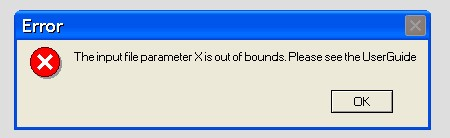
\includegraphics[width=0.6\textwidth]{errorMessage.jpeg}
\caption{Input out of Bounds}
\label{Fig_InputError}
\end{center}
\end{figure}

Test Case Derivation: 
I (individual inputs) are an element of V. P(V) is incorrect if P:V and at least one I is out of bounds as per Table \ref{table:inputdatabounds}: Input Data Bounds. This test satisfies R3.\\ 

					
How test will be performed: 

\begin{enumerate}
\item Outside of the system, the input values will be written to a comma delimited text file titled input.txt, as outlined in the User Guide (\citet{LBM_UserGuide_PM}).
\item The file will be placed into the Input directory, under the home directory of the project.
\item The module TestInput found under the home directory will be run using a python IDE.
\item If the test is successful, the system will output a descriptive error message, as seen above, to the screen.\\


\end{enumerate}

\end{enumerate}

~\newpage

\subsubsection{Von Karman Vortex Street}
\label{frvkvs}
		
\paragraph{Dynamic Testing - Manual:}
\paragraph{} These dynamic tests will compare {\myprogname} output with output from the pseudo-oracle myLBM (\citet{pylbmcode}). The pseudo-oracle will have the same inputs as {\myprogname} for each test. The allowable error is AVERAGE\_ERROR, found in Section \ref{symbolpara}.

\begin{enumerate}

\item{tutorial-test-id3\\}

Control: Program (P) module execution using inputs (V), and expecting output (O) to match a control value (C).\\
					
Initial State: No input file in Input directory.\\
					
Input: A comma delimited file, with inputs marked in the manner outlined in the User Guide (\citet{LBM_UserGuide_PM}).\\The input values for this test will be:\\
$Re$: 500\\
$t$: 75\\
$\rho$: 1.0\\
$\eta_b$: 1.e-3\\
$X_{min}$ = 0.\\
$X_{max}$ = 3.\\
$Y_{min}$ = 0.\\
$Y_{max}$ = 1.\\
$R$ = 0.05\\
$\mathrm{e_{sch}}$ = 1.\\
$\mathrm{e_{fac}}$ = 20\\
$S$ = 64\\
$\mathrm{D}$ = 2\\
$\mathrm{Q}$ = 9\\

		
Output: Vorticity vector values printed to the screen. \\

Test Case Derivation: This case is a comparison with the pseudo-oracle pyLBM. The output vector values (C) of this test for pyLBM can be found in the file id3output.txt located in the OracleOutput folder. The result required for the test to pass is an average error rate between cells of the output vector (O) and (C) of less than or equal to AVERAGE\_ERROR.\\


How test will be performed: 

\begin{enumerate}
\item The Von Karman Vortex Street module shall be modified by the author to print the vorticity vector as output.
\item Outside of the system, the input parameter values will be written to a comma delimited text file titled input.txt, as outlined in the User Guide.
\item The file will be placed into the Input directory, under the home directory of the project.
\item The module for Von Karman Vortex Street will be selected to run.
\item Upon completion of the module, the output values of the vorticity vector will be compared to the vorticity vector values from pyLBM - comparison will be done per cell. Comparisons can be done manually using Excel, or through a script.\\
\end{enumerate}

\item{Reynolds-Rel-Error-test-id4\\}

Control: Program (P) module execution using  inputs (V) with varying $Re$ parameter (I), and observing variance of the relative error ($E_r$) of the output (O) when compared to a control value (C) \\
					
Initial State: No input file in Input directory.\\
					
Input (first iteration of test): A comma delimited file, with inputs marked in the manner outlined in the User Guide (\citet{LBM_UserGuide_PM}).\\The input values for this test will be:\\
$Re$: 500\\
$t$: 75\\
$\rho$: 1.0\\
$\eta_b$: 1.e-3\\
$X_{min}$ = 0.\\
$X_{max}$ = 3.\\
$Y_{min}$ = 0.\\
$Y_{max}$ = 1.\\
$R$ = 0.05\\
$\mathrm{e_{sch}}$ = 1.\\
$\mathrm{e_{fac}}$ = 20\\
$S$ = 64\\
$\mathrm{D}$ = 2\\
$\mathrm{Q}$ = 9\\

Input (second iteration of test): A comma delimited file, with inputs marked in the manner outlined in the User Guide (\citet{LBM_UserGuide_PM}).\\The input values for this test will be:\\
$Re$: 1500\\
$t$: 75\\
$\rho$: 1.0\\
$\eta_b$: 1.e-3\\
$X_{min}$ = 0.\\
$X_{max}$ = 3.\\
$Y_{min}$ = 0.\\
$Y_{max}$ = 1.\\
$R$ = 0.05\\
$\mathrm{e_{sch}}$ = 1.\\
$\mathrm{e_{fac}}$ = 20\\
$S$ = 64\\
$\mathrm{D}$ = 2\\
$\mathrm{Q}$ = 9\\

Input (third iteration of test): A comma delimited file, with inputs marked in the manner outlined in the User Guide (\citet{LBM_UserGuide_PM}).\\The input values for this test will be:\\
$Re$: 2500\\
$t$: 75\\
$\rho$: 1.0\\
$\eta_b$: 1.e-3\\
$X_{min}$ = 0.\\
$X_{max}$ = 3.\\
$Y_{min}$ = 0.\\
$Y_{max}$ = 1.\\
$R$ = 0.05\\
$\mathrm{e_{sch}}$ = 1.\\
$\mathrm{e_{fac}}$ = 20\\
$S$ = 64\\
$\mathrm{D}$ = 2\\
$\mathrm{Q}$ = 9\\

		
Output: In each iteration we will have vorticity vector values printed to the screen.\\

Test Case Derivation: This case is a comparison with the pseudo-oracle pyLBM. The C values of this test for pyLBM can be found in the files id4\_1\_output.txt, id4\_2\_output.txt and id4\_3\_output.txt, located in the OracleOutput folder. The files hold the C values for iterations 1, 2, and 3 respectively. Each iteration will calculate the relative error of O to its respective C counterpart. The $E_r$ values of the iterations will be compared with the intent to discover how changes in $Re$ affect correctness. This may be helpful in improving correctness of the implementation.\\	

How test will be performed: 

\begin{enumerate}
\item The Von Karman Vortex Street module shall be modified by the author to print the vorticity vector as output.
\item Outside of the system, the input parameter values will be written to a comma delimited text file titled input.txt, as outlined in the User Guide.
\item The file will be placed into the Input directory, under the home directory of the project.
\item The module for Von Karman Vortex Street will be selected to run.
\item Upon completion of the module, the output values of the vorticity vector will be compared to the vorticity vector values from pyLBM - comparison will be done per cell. Comparisons can be done manually using Excel, or through a script. A relative error value will be calculated.\\
\item Steps (a) - (e) will be repeated for each test iteration.
\item The $E_r$ of each iteration will be compared.\\
\end{enumerate}
					
\item{laminar-test-id5\\}

Control: Program (P) module execution using inputs (V), and expecting output (O) to match a control value (C).\\
					
Initial State: No input file in Input directory.\\
					
A comma delimited file, with inputs marked in the manner outlined in the User Guide (\citet{LBM_UserGuide_PM}).\\The input values for this test will be:\\
$Re$: 0.0001\\
$t$: 75\\
$\rho$: 1.0\\
$\eta_b$: 1.e-3\\
$X_{min}$ = 0.\\
$X_{max}$ = 3.\\
$Y_{min}$ = 0.\\
$Y_{max}$ = 1.\\
$R$ = 0.05\\
$\mathrm{e_{sch}}$ = 1.\\
$\mathrm{e_{fac}}$ = 20\\
$S$ = 64\\
$\mathrm{D}$ = 2\\
$\mathrm{Q}$ = 9\\
					
Output: Vorticity vector values printed to the screen.\\

Test Case Derivation: This case is a comparison with the pseudo-oracle pyLBM. The C values of this test for pyLBM can be found in the file id5output.txt located in the OracleOutput folder. The result required for the test to pass is an average error rate between cells of O and C of less than or equal to AVERAGE\_ERROR.\\
This test covers a very small Reynolds number representing laminar flow.\\	

					
How test will be performed: 

\begin{enumerate}
\item The Von Karman Vortex Street module shall be modified by the author to print the vorticity vector as output.
\item Outside of the system, the input parameter values will be written to a comma delimited text file titled input.txt, as outlined in the User Guide.
\item The file will be placed into the Input directory, under the home directory of the project.
\item The module for Von Karman Vortex Street will be selected to run.
\item Upon completion of the module, the output values of the vorticity vector will be compared to the vorticity vector values from pyLBM - comparison will be done per cell. Comparisons can be done manually using Excel, or through a script.\\
\end{enumerate}

\item{turbulent-test-id6\\}

Control: Program (P) module execution using inputs (V), and expecting output (O) to match a control value (C).\\
					
Initial State: No input file in Input directory.\\
					
A comma delimited file, with inputs marked in the manner outlined in the User Guide (\citet{LBM_UserGuide_PM}).\\The input values for this test will be:\\
$Re$: 50000\\
$t$: 75\\
$\rho$: 1.0\\
$\eta_b$: 1.e-3\\
$X_{min}$ = 0.\\
$X_{max}$ = 3.\\
$Y_{min}$ = 0.\\
$Y_{max}$ = 1.\\
$R$ = 0.05\\
$\mathrm{e_{sch}}$ = 1.\\
$\mathrm{e_{fac}}$ = 20\\
$S$ = 64\\
$\mathrm{D}$ = 2\\
$\mathrm{Q}$ = 9\\

Output: Vorticity vector values printed to the screen. \\

Test Case Derivation: This case is a comparison with the pseudo-oracle pyLBM. The C values of this test for pyLBM can be found in the file id6output.txt located in the OracleOutput folder. The result required for the test to pass is an average error rate between O and C of less than or equal to AVERAGE\_ERROR.\\
This test covers a very large Reynolds number representing very turbulent flow.\\	

					
How test will be performed: 

\begin{enumerate}
\item The Von Karman Vortex Street module shall be modified by the author to print the vorticity vector as output.
\item Outside of the system, the input parameter values will be written to a comma delimited text file titled input.txt, as outlined in the User Guide.
\item The file will be placed into the Input directory, under the home directory of the project.
\item The module for Von Karman Vortex Street will be selected to run.
\item Upon completion of the module, the output values of the vorticity vector will be compared to the vorticity vector values from pyLBM - comparison will be done per cell. Comparisons can be done manually using Excel, or through a script.\\
\end{enumerate}

\item{low-density-test-id7\\}

Control: Program (P) module execution using inputs (V), and expecting output (O) to match a control value (C).\\
					
Initial State: No input file in Input directory.\\
					
A comma delimited file, with inputs marked in the manner outlined in the User Guide (\citet{LBM_UserGuide_PM}).\\The input values for this test will be:\\
$Re$: 500\\
$t$: 75\\
$\rho$: 7.08e-2\\
$\eta_b$: 1.e-3\\
$X_{min}$ = 0.\\
$X_{max}$ = 3.\\
$Y_{min}$ = 0.\\
$Y_{max}$ = 1.\\
$R$ = 0.05\\
$\mathrm{e_{sch}}$ = 1.\\
$\mathrm{e_{fac}}$ = 20\\
$S$ = 64\\
$\mathrm{D}$ = 2\\
$\mathrm{Q}$ = 9\\

Output: Vorticity vector values printed to the screen. \\

Test Case Derivation: This case is a comparison with the pseudo-oracle pyLBM. The C values of this test for pyLBM can be found in the file id7output.txt located in the OracleOutput folder. The result required for the test to pass is an average error rate between O and C of less than or equal to AVERAGE\_ERROR.\\
This test covers the low bound for density using a density of liquid hydrogen.\\

					
How test will be performed: 

\begin{enumerate}
\item The Von Karman Vortex Street module shall be modified by the author to print the vorticity vector as output.
\item Outside of the system, the input parameter values will be written to a comma delimited text file titled input.txt, as outlined in the User Guide.
\item The file will be placed into the Input directory, under the home directory of the project.
\item The module for Von Karman Vortex Street will be selected to run.
\item Upon completion of the module, the output values of the vorticity vector will be compared to the vorticity vector values from pyLBM - comparison will be done per cell. Comparisons can be done manually using Excel, or through a script.\\
\end{enumerate}

\item{high-density-test-id8\\}

Control: Program (P) module execution using inputs (V), and expecting output (O) to match a control value (C).\\
					
Initial State: No input file in Input directory.\\
					
A comma delimited file, with inputs marked in the manner outlined in the User Guide (\citet{LBM_UserGuide_PM}).\\The input values for this test will be:\\
$Re$: 500\\
$t$: 75\\
$\rho$: 13.6\\
$\eta_b$: 1.e-3\\
$X_{min}$ = 0.\\
$X_{max}$ = 3.\\
$Y_{min}$ = 0.\\
$Y_{max}$ = 1.\\
$R$ = 0.05\\
$\mathrm{e_{sch}}$ = 1.\\
$\mathrm{e_{fac}}$ = 20\\
$S$ = 64\\
$\mathrm{D}$ = 2\\
$\mathrm{Q}$ = 9\\

Output: Vorticity vector values printed to the screen. \\

Test Case Derivation: This case is a comparison with the pseudo-oracle pyLBM. The C values of this test for pyLBM can be found in the file id8output.txt located in the OracleOutput folder. The result required for the test to pass is an average error rate between O and C of less than or equal to AVERAGE\_ERROR.\\
This test covers the high bound for density using a density close to that of mercury.\\

					
How test will be performed: 

\begin{enumerate}
\item The Von Karman Vortex Street module shall be modified by the author to print the vorticity vector as output.
\item Outside of the system, the input parameter values will be written to a comma delimited text file titled input.txt, as outlined in the User Guide.
\item The file will be placed into the Input directory, under the home directory of the project.
\item The module for Von Karman Vortex Street will be selected to run.
\item Upon completion of the module, the output values of the vorticity vector will be compared to the vorticity vector values from pyLBM - comparison will be done per cell. Comparisons can be done manually using Excel, or through a script.\\
\end{enumerate}

\item{low-bulk-viscosity-test-id9\\}

Control: Program (P) module execution using inputs (V), and expecting output (O) to match a control value (C).\\
					
Initial State: No input file in Input directory.\\
					
A comma delimited file, with inputs marked in the manner outlined in the User Guide (\citet{LBM_UserGuide_PM}).\\The input values for this test will be:\\
$Re$: 500\\
$t$: 75\\
$\rho$: 1.0\\
$\eta_b$: 1.e-4\\
$X_{min}$ = 0.\\
$X_{max}$ = 3.\\
$Y_{min}$ = 0.\\
$Y_{max}$ = 1.\\
$R$ = 0.05\\
$\mathrm{e_{sch}}$ = 1.\\
$\mathrm{e_{fac}}$ = 20\\
$S$ = 64\\
$\mathrm{D}$ = 2\\
$\mathrm{Q}$ = 9\\

Output: Vorticity vector values printed to the screen.  \\

Test Case Derivation: This case is a comparison with the pseudo-oracle pyLBM. The C values of this test for pyLBM can be found in the file id9output.txt located in the OracleOutput folder. The result required for the test to pass is an average error rate between O and C of less than or equal to AVERAGE\_ERROR.\\
This test covers the low bound for bulk viscosity.\\

					
How test will be performed: 

\begin{enumerate}
\item The Von Karman Vortex Street module shall be modified by the author to print the vorticity vector as output.
\item Outside of the system, the input parameter values will be written to a comma delimited text file titled input.txt, as outlined in the User Guide.
\item The file will be placed into the Input directory, under the home directory of the project.
\item The module for Von Karman Vortex Street will be selected to run.
\item Upon completion of the module, the output values of the vorticity vector will be compared to the vorticity vector values from pyLBM - comparison will be done per cell. Comparisons can be done manually using Excel, or through a script.\\
\end{enumerate}

\item{high-bulk-viscosity-test-id10\\}

Control: Program (P) module execution using inputs (V), and expecting output (O) to match a control value (C).\\
					
Initial State: No input file in Input directory.\\
					
A comma delimited file, with inputs marked in the manner outlined in the User Guide (\citet{LBM_UserGuide_PM}).\\The input values for this test will be:\\
$Re$: 500\\
$t$: 75\\
$\rho$: 1.0\\
$\eta_b$: 1.e-2\\
$X_{min}$ = 0.\\
$X_{max}$ = 3.\\
$Y_{min}$ = 0.\\
$Y_{max}$ = 1.\\
$R$ = 0.05\\
$\mathrm{e_{sch}}$ = 1.\\
$\mathrm{e_{fac}}$ = 20\\
$S$ = 64\\
$\mathrm{D}$ = 2\\
$\mathrm{Q}$ = 9\\

Output: Vorticity vector values printed to the screen. \\ 

Test Case Derivation: This case is a comparison with the pseudo-oracle pyLBM. The C values of this test for pyLBM can be found in the file id10output.txt located in the OracleOutput folder. The result required for the test to pass is an average error rate between O and C of less than or equal to AVERAGE\_ERROR.\\
This test covers the high bound for bulk viscosity.\\

					
How test will be performed: 

\begin{enumerate}
\item The Von Karman Vortex Street module shall be modified by the author to print the vorticity vector as output.
\item Outside of the system, the input parameter values will be written to a comma delimited text file titled input.txt, as outlined in the User Guide.
\item The file will be placed into the Input directory, under the home directory of the project.
\item The module for Von Karman Vortex Street will be selected to run.
\item Upon completion of the module, the output values of the vorticity vector will be compared to the vorticity vector values from pyLBM - comparison will be done per cell. Comparisons can be done manually using Excel or through a script.\\
\end{enumerate}

\end{enumerate}
~\newpage

\subsubsection{Poiseuille Flow}
\label{frpf}

\paragraph{Dynamic Testing - Manual:}
\paragraph{} These dynamic tests will compare {\myprogname} output with output from the pseudo oracle myLBM (\citet{pylbmcode}). The input oracle will have the same inputs as {\myprogname} for each test. The allowable error is AVERAGE\_ERROR, found in Section \ref{symbolpara}.

\begin{enumerate}

\item{tutorial-test-id11\\}

Control: Program (P) module execution using inputs (V), and expecting output (O) to match a control value (C).\\
					
Initial State: No input file in Input directory.\\
					
A comma delimited file, with inputs marked in the manner outlined in the User Guide (\citet{LBM_UserGuide_PM}).\\The input values for this test will be:\\
$t$: 50\\
$\rho$: 1\\
$\eta_b$: 1.e-2\\
$\eta_s$: 1.e-2\\
$S$ = 16\\
$D_{l}$ = 2\\
$D_{w}$ = 1\\
$\mathrm{e_{sch}}$ = 1.\\
$\mathrm{e_{max}}$ = 0.1\\
$X_{min}$ = 0.\\

					
Output: Pressure gradient value printed to the screen.  \\

Test Case Derivation: This case is a comparison with the pseudo-oracle pyLBM, which has a module for Poiseuille Flow. The output pressure gradient value of this test is to be compared to the C value from the pseudo-oracle, -7.074e-03. The result required for the test to pass is an average error rate between O and C of less than or equal to AVERAGE\_ERROR.\\

					
How test will be performed: 

\begin{enumerate}
\item Outside of the system, the input parameter values will be written to a comma delimited text file titled input.txt, as outlined in the User Guide.
\item The file will be placed into the Input directory, under the home directory of the project.
\item The module for Poiseuille Flow will be selected to run.
\item Upon completion of the module, the pressure gradient output value will be compared to the above output value from the pseudo-oracle.
\end{enumerate}			

\item{low-density-test-id12\\}

Control: Program (P) module execution using inputs (V), and expecting output (O) to match a control value (C).\\
					
Initial State: No input file in Input directory.\\
					
A comma delimited file, with inputs marked in the manner outlined in the User Guide (\citet{LBM_UserGuide_PM}).\\The input values for this test will be:\\
$t$: 50\\
$\rho$: 0.0708\\
$\eta_b$: 1.e-2\\
$\eta_s$: 1.e-2\\
$S$ = 16\\
$D_{l}$ = 2\\
$D_{w}$ = 1\\
$\mathrm{e_{sch}}$ = 1.\\
$\mathrm{e_{max}}$ = 0.1\\
$X_{min}$ = 0.\\

					
Output: Pressure gradient value printed to the screen. \\ 

Test Case Derivation: This case is a comparison with the pseudo-oracle pyLBM, which has a module for Poiseuille Flow. The output pressure gradient value of this test is to be compared to the C value from the pseudo-oracle, -4.103e-03. The result required for the test to pass is an average error rate between O and C of less than or equal to AVERAGE\_ERROR.\\

					
How test will be performed: 

\begin{enumerate}
\item Outside of the system, the input parameter values will be written to a comma delimited text file titled input.txt, as outlined in the User Guide.
\item The file will be placed into the Input directory, under the home directory of the project.
\item The module for Poiseuille Flow will be selected to run.
\item Upon completion of the module, the pressure gradient output value will be compared to the above output value from the pseudo-oracle.
\end{enumerate}	

\item{high-density-test-id13\\}

Control: Program (P) module execution using inputs (V), and expecting output (O) to match a control value (C).\\
					
Initial State: No input file in Input directory.\\
					
A comma delimited file, with inputs marked in the manner outlined in the User Guide (\citet{LBM_UserGuide_PM}).\\The input values for this test will be:\\
$t$: 50\\
$\rho$: 13.6\\
$\eta_b$: 1.e-2\\
$\eta_s$: 1.e-2\\
$S$ = 16\\
$D_{l}$ = 2\\
$D_{w}$ = 1\\
$\mathrm{e_{sch}}$ = 1.\\
$\mathrm{e_{max}}$ = 0.1\\
$X_{min}$ = 0.\\

					
Output: Pressure gradient value printed to the screen.  \\

Test Case Derivation: This case is a comparison with the pseudo-oracle pyLBM, which has a module for Poiseuille Flow. The output pressure gradient value of this test is to be compared to the C value from the pseudo-oracle, -1.522e-01. The result required for the test to pass is an average error rate between O and C of less than or equal to AVERAGE\_ERROR.\\

					
How test will be performed: 

\begin{enumerate}
\item Outside of the system, the input parameter values will be written to a comma delimited text file titled input.txt, as outlined in the User Guide.
\item The file will be placed into the Input directory, under the home directory of the project.
\item The module for Poiseuille Flow will be selected to run.
\item Upon completion of the module, the pressure gradient output value will be compared to the above output value from the pseudo-oracle.
\end{enumerate}	

\item{low-bulk-viscosity-test-id14\\}

Control: Program (P) module execution using inputs (V), and expecting output (O) to match a control value (C).\\
					
Initial State: No input file in Input directory.\\
					
A comma delimited file, with inputs marked in the manner outlined in the User Guide (\citet{LBM_UserGuide_PM}).\\The input values for this test will be:\\
$t$: 50\\
$\rho$: 1\\
$\eta_b$: 1.e-4\\
$\eta_s$: 1.e-2\\
$S$ = 16\\
$D_{l}$ = 2\\
$D_{w}$ = 1\\
$\mathrm{e_{sch}}$ = 1.\\
$\mathrm{e_{max}}$ = 0.1\\
$X_{min}$ = 0.\\

					
Output: Pressure gradient value printed to the screen. \\ 

Test Case Derivation: This case is a comparison with the pseudo-oracle pyLBM, which has a module for Poiseuille Flow. The output pressure gradient value of this test is to be compared to the C output from the pseudo-oracle, -1.462e-01. The result required for the test to pass is an average error rate between O and C of less than or equal to AVERAGE\_ERROR.\\

					
How test will be performed: 

\begin{enumerate}
\item Outside of the system, the input parameter values will be written to a comma delimited text file titled input.txt, as outlined in the User Guide.
\item The file will be placed into the Input directory, under the home directory of the project.
\item The module for Poiseuille Flow will be selected to run.
\item Upon completion of the module, the pressure gradient output value will be compared to the above output value from the pseudo-oracle.
\end{enumerate}	

\item{high-bulk-viscosity-test-id15\\}

Control: Program (P) module execution using inputs (V), and expecting output (O) to match a control value (C).\\
					
Initial State: No input file in Input directory.\\
					
A comma delimited file, with inputs marked in the manner outlined in the User Guide (\citet{LBM_UserGuide_PM}).\\The input values for this test will be:\\
$t$: 50\\
$\rho$: 1\\
$\eta_b$: 20000\\
$\eta_s$: 1.e-2\\
$S$ = 16\\
$D_{l}$ = 2\\
$D_{w}$ = 1\\
$\mathrm{e_{sch}}$ = 1.\\
$\mathrm{e_{max}}$ = 0.1\\
$X_{min}$ = 0.\\

					
Output: Pressure gradient value printed to the screen.  \\

Test Case Derivation: This case is a comparison with the pseudo-oracle pyLBM, which has a module for Poiseuille Flow. The output pressure gradient value of this test is to be compared to the C value from the pseudo-oracle, -3.262e-03. The result required for the test to pass is an average error rate between O and C of less than or equal to AVERAGE\_ERROR.\\

					
How test will be performed: 

\begin{enumerate}
\item Outside of the system, the input parameter values will be written to a comma delimited text file titled input.txt, as outlined in the User Guide.
\item The file will be placed into the Input directory, under the home directory of the project.
\item The module for Poiseuille Flow will be selected to run.
\item Upon completion of the module, the pressure gradient output value will be compared to the above output value from the pseudo-oracle.
\end{enumerate}	

\item{low-shear-viscosity-test-id16\\}

Control: Program (P) module execution using inputs (V), and expecting output (O) to match a control value (C).\\
					
Initial State: No input file in Input directory.\\
					
A comma delimited file, with inputs marked in the manner outlined in the User Guide (\citet{LBM_UserGuide_PM}).\\The input values for this test will be:\\
$t$: 50\\
$\rho$: 1\\
$\eta_b$: 1.e-2\\
$\eta_s$: 1.e-3\\
$S$ = 16\\
$D_{l}$ = 2\\
$D_{w}$ = 1\\
$\mathrm{e_{sch}}$ = 1.\\
$\mathrm{e_{max}}$ = 0.1\\
$X_{min}$ = 0.\\

					
Output: Pressure gradient value printed to the screen. \\ 

Test Case Derivation: This case is a comparison with the pseudo-oracle pyLBM, which has a module for Poiseuille Flow. The output pressure gradient value of this test is to be compared to the C value from the pseudo-oracle, -1.604e-03. The result required for the test to pass is an average error rate between O and C of less than or equal to AVERAGE\_ERROR.\\

					
How test will be performed: 

\begin{enumerate}
\item Outside of the system, the input parameter values will be written to a comma delimited text file titled input.txt, as outlined in the User Guide.
\item The file will be placed into the Input directory, under the home directory of the project.
\item The module for Poiseuille Flow will be selected to run.
\item Upon completion of the module, the pressure gradient output value will be compared to the above output value from the pseudo-oracle.
\end{enumerate}	

\item{high-shear-viscosity-test-id17\\}

Control: Program (P) module execution using inputs (V), and expecting output (O) to match a control value (C).\\
					
Initial State: No input file in Input directory.\\
					
A comma delimited file, with inputs marked in the manner outlined in the User Guide (\citet{LBM_UserGuide_PM}).\\The input values for this test will be:\\
$t$: 50\\
$\rho$: 1\\
$\eta_b$: 1.e-2\\
$\eta_s$: 20000\\
$S$ = 16\\
$D_{l}$ = 2\\
$D_{w}$ = 1\\
$\mathrm{e_{sch}}$ = 1.\\
$\mathrm{e_{max}}$ = 0.1\\
$X_{min}$ = 0.\\

					
Output: Pressure gradient value printed to the screen. \\ 

Test Case Derivation: This case is a comparison with the pseudo-oracle pyLBM, which has a module for Poiseuille Flow. The output pressure gradient value of this test is to be compared to the C value from the pseudo-oracle, -6.868e-01. The result required for the test to pass is an average error rate between O and C of less than or equal to AVERAGE\_ERROR.\\

					
How test will be performed: 

\begin{enumerate}
\item Outside of the system, the input parameter values will be written to a comma delimited text file titled input.txt, as outlined in the User Guide.
\item The file will be placed into the Input directory, under the home directory of the project.
\item The module for Poiseuille Flow will be selected to run.
\item Upon completion of the module, the pressure gradient output value will be compared to the above output value from the pseudo-oracle.
\end{enumerate}	

\end{enumerate}

~\newpage

\subsection{Tests for Nonfunctional Requirements}
\label{nfrtest}

\subsubsection{Correctness}

System correctness is tested via the functional tests of Section \ref{testfr} using an allowable AVERAGE\_ERROR as stated in Section \ref{symbolpara}.

\subsubsection{Maintainability}
		
\paragraph{Document Walkthrough}

\begin{enumerate}

\item{maintainability-id18\\}

Type: Maintainability Walkthrough\\
					
Initial State: Maintainability of the repository has not been tested.\\
					
Input/Condition: A production version of {\myprogname} has been released.\\
					
Output/Result: A graded report describing the maintainability of the repository.\\

Test Case Derivation: This test will determine if the system documentation allows for easy maintainability by checking how much documentation is available, as well as reviewing its clarity and traceability. A score of higher than 3 in each of the tested categories will indicate that the system documentation is maintainable.\\ 
					
How test will be performed: 

\begin{enumerate}
\item Ao Dong shall check the repository for the following documentation: SRS/CA, VnV Plan, MG, MIS, User Guide.
\item Ao Dong shall mark 1 point for each of the above documents.
\item Ao Dong shall read through each of the above documents and provide a grade between 1 and 5 for clarity of the writing. A score of 1 represents a document that is hard to understand, and a score of 5 represents a document that is easy to understand. The user shall divide the sum of the scores for all of the reports by 5.
\item Ao Dong shall read through each of the above documents and provide a grade between 1 and 5 for traceability within the document. A score of 1 represents no links within the report, and a score of 5 represents many links between sections of the report. The user shall then divide the sum of the scores for all of the reports by 5.
\item Ao Dong will generate a brief report with the above three values, from steps (c) to (e).\\
\end{enumerate}

\end{enumerate}

\subsubsection{Performance}
		
\paragraph{Running Time}

\begin{enumerate}

\item{performance-id19\\}

Type: Running Time\\
					
Initial State: Input file is in the appropriate directory. The file contains the required parameter values for 2 different modules - Von Karman Vortex Street and Poiseuille Flow.\\
					
Input/Condition: A comma delimited file with the following input parameters and values:\\
$Re$: 500\\
$t$: 200\\
$\rho$: 1.0\\
$\eta_b$: 1.e-3\\
$X_{min}$ = 0.\\
$X_{max}$ = 3.\\
$Y_{min}$ = 0.\\
$Y_{max}$ = 1.\\
$R$ = 0.05\\
$\mathrm{e_{sch}}$ = 1.\\
$\mathrm{e_{fac}}$ = 20\\
$S$ = 64\\
$\mathrm{D}$ = 2\\
$\mathrm{Q}$ = 9\\
					
Output/Result: A timed comparison of running
each of the two system modules, Von Karman Vortex Street and Poiseuille Flow, against the psuedo-oracle pyLBM using pyCharm IDE. The test will be passed if both system modules are faster than the pseudo-oracle.\\

How test will be performed: 

\begin{enumerate}
\item Outside of the system, the input parameter values will be written, by the author, to a comma delimited text file titled input.txt, as outlined in the User Guide.
\item The file will be placed into the Input directory, under the home directory of the project.
\item The author shall first start a timer and then select the Poiseuille Flow module to run.
\item Upon completion of the module the author shall note the module running time.
\item The author shall repeat steps (c) to (d) for the Von Karman Vortex Street module. 
\item The author shall then run each of the problems, Poiseuille Flow and Von Karman Vortex Street, using the pseudo-oralce pyLBM using pyCharm IDE, making sure to time the running of each problem.
\item The author shall compare the running time of each of the two system modules, Von Karman Vortex Street and Poiseuille Flow, against the psuedo-oracle.\\
\end{enumerate}

\end{enumerate}

\subsubsection{Portability}
		
\paragraph{Operating System Portability}

\begin{enumerate}

\item{portability-id20\\}

Type: Portability Check\\
					
Initial State: Have PyCharm IDE installed on three separate operating systems (virtual machines can be used for this): macOS, Windows, Linux. \\
					
Input/Condition: A comma delimited file with the following input parameters and values:\\
$Re$: 500\\
$t$: 75\\
$\rho$: 1.0\\
$\eta_b$: 1.e-3\\
$X_{min}$ = 0.\\
$X_{max}$ = 3.\\
$Y_{min}$ = 0.\\
$Y_{max}$ = 1.\\
$R$ = 0.05\\
$\mathrm{e_{sch}}$ = 1.\\
$\mathrm{e_{fac}}$ = 20\\
$S$ = 64\\
$\mathrm{D}$ = 2\\
$\mathrm{Q}$ = 9\\

					
Output/Result: This case is a check of the ability of the LBM solution to run on multiple operating systems. The result required for the test to pass is a vorticity vector printed to the screen of each instance which matches, within the allowable AVERAGE\_ERROR, the vorticity vector value found in the file id20output.txt located in the OracleOutput folder.\\
					
How test will be performed: 

\begin{enumerate}

\item The input parameter values will be written, by the author, to a comma delimited text file titled input.txt, as outlined in the User Guide.
\item The file will be placed into the Input directory, under the home directory of the project, in each of the operating system instances.
\item The Von Karman Vortex Street module shall be modified by the author to print the vorticity vector as output.
\item The author shall run the Von Karman Vortex Street module.
\item Upon completion of the module, the author will compare the output values of the vorticity vector to the vorticity vector values of the pseudo-oracle.\\
\end{enumerate}

\end{enumerate}

\subsubsection{Robustness}
		
System robustness is tested through the Input Bounds test (input-bounds-id2) in Section \ref{testfr}.

\subsubsection{Usability}

\paragraph{Usability Survey}

\begin{enumerate}

\item{usability-id21\\}

Type: Usability Survey\\
					
Initial State: The {\myprogname} repository, the below input parameters, and an instruction to run the Von Karman Vortex Street module are provided to three anonymous users via GitHub.\\
					
Input/Condition: A usability survey with the questions listed in Section \ref{usabilitysurevyquestions} and a comma delimited file with the following input parameters and values:\\
$Re$: 500\\
$t$: 75\\
$\rho$: 1.0\\
$\eta_b$: 1.e-3\\
$X_{min}$ = 0.\\
$X_{max}$ = 3.\\
$Y_{min}$ = 0.\\
$Y_{max}$ = 1.\\
$R$ = 0.05\\
$\mathrm{e_{sch}}$ = 1.\\
$\mathrm{e_{fac}}$ = 20\\
$S$ = 64\\
$\mathrm{D}$ = 2\\
$\mathrm{Q}$ = 9\\

				
Output/Result: Survey results.\\

Test Case Derivation: This case is a check of the usability of the LBM solver. Respondents will be asked to rank their experience of running a module. A final average grade of higher than 3 will indicate that the users found the system to be user friendly.\\
	
How test will be performed: 

\begin{enumerate}
\item Each participant will be instructed to run a Von Karman Vortex Street simulation using the provided input parameters.
\item The participants will attempt to run the simulation.
\item Upon completion of the attempt, the participants will be asked to answer the survey questions.
\item The questionnaire results will be tallied and averaged.
\end{enumerate}

\end{enumerate}

~\newpage
\subsection{Traceability Between Test Cases and Requirements}

\begin{table}[!h]
\begin{center}
\begin{tabular}{| c | c | c | c | c | c | c | c |}
\hline
& R1 & R2 & R3 & R4 & R5 & R6 & R7\\
\hline
id1 & \checkmark & & & & & &\\
\hline
id2 & & & \checkmark & & & &\\
\hline
id3 & \checkmark & \checkmark & \checkmark & \checkmark & \checkmark & \checkmark & \checkmark \\
\hline
id4 & \checkmark & \checkmark & \checkmark & \checkmark & \checkmark & \checkmark & \checkmark \\
\hline
id5 & \checkmark & \checkmark & \checkmark & \checkmark & \checkmark & \checkmark & \checkmark \\
\hline
id6 & \checkmark & \checkmark & \checkmark & \checkmark & \checkmark & \checkmark & \checkmark \\
\hline
id7 & \checkmark & \checkmark & \checkmark & \checkmark & \checkmark & \checkmark & \checkmark \\
\hline
id8 & \checkmark & \checkmark & \checkmark & \checkmark & \checkmark & \checkmark & \checkmark \\
\hline
id9 & \checkmark & \checkmark & \checkmark & \checkmark & \checkmark & \checkmark & \checkmark \\
\hline
id10 & \checkmark & \checkmark & \checkmark & \checkmark & \checkmark & \checkmark & \checkmark \\
\hline
id11 & \checkmark & \checkmark & \checkmark & \checkmark & \checkmark & \checkmark & \checkmark \\
\hline
id12 & \checkmark & \checkmark & \checkmark & \checkmark & \checkmark & \checkmark & \checkmark \\
\hline
id13 & \checkmark & \checkmark & \checkmark & \checkmark & \checkmark & \checkmark & \checkmark \\
\hline
id14 & \checkmark & \checkmark & \checkmark & \checkmark & \checkmark & \checkmark & \checkmark \\
\hline
id15 & \checkmark & \checkmark & \checkmark & \checkmark & \checkmark & \checkmark & \checkmark \\
\hline
id16 & \checkmark & \checkmark & \checkmark & \checkmark & \checkmark & \checkmark & \checkmark \\
\hline
id17 & \checkmark & \checkmark & \checkmark & \checkmark & \checkmark & \checkmark & \checkmark \\
\hline
id18 & & & & & & & \\
\hline
id19 & \checkmark & \checkmark & \checkmark & \checkmark & \checkmark & \checkmark & \checkmark \\
\hline
id20 & \checkmark & \checkmark & \checkmark & \checkmark & \checkmark & \checkmark & \checkmark \\
\hline
id21 & \checkmark & \checkmark & \checkmark & \checkmark & \checkmark & \checkmark & \checkmark \\
\hline
\end{tabular}
\caption{Traceability Matrix Showing the Connections Between Test Cases and Functional Requirements}
\end{center}
\end{table}   

\begin{table}[!h]
\begin{center}
\begin{tabular}{| c | c | c | c | c | c | c | c | c | c | c |}
\hline
Cases / NFR & 1 & 2 & 3 & 4 & 5 & 6 & 7 & 8 & 9 & 10\\
\hline
id1 & & & & & & & & & &\\
\hline
id2 & & & & & & & \checkmark & & &\\
\hline
id3 & \checkmark & & & & & & & & &\\
\hline
id4 & & & & & & & & & &\\
\hline
id5 & \checkmark & & & & & & & & &\\
\hline
id6 & \checkmark & & & & & & & & &\\
\hline
id7 & \checkmark & & & & & & & & &\\
\hline
id8 & \checkmark & & & & & & & & &\\
\hline
id9 & \checkmark & & & & & & & & &\\
\hline
id10 & \checkmark & & & & & & & & &\\
\hline
id11 & \checkmark & & & & & & & & &\\
\hline
id12 & \checkmark & & & & & & & & &\\
\hline
id13 & \checkmark & & & & & & & & &\\
\hline
id14 & \checkmark & & & & & & & & &\\
\hline
id15 & \checkmark & & & & & & & & &\\
\hline
id16 & \checkmark & & & & & & & & &\\
\hline
id17 & \checkmark & & & & & & & & &\\
\hline
id18 & & \checkmark & & & & & & & &\\
\hline
id19 & & & \checkmark & & & & & & &\\
\hline
id20 & \checkmark & & & \checkmark & & & & & &\\
\hline
id21 & & & & & & & & & & \checkmark \\
\hline
\end{tabular}
\caption{Traceability Matrix Showing the Connections Between Test Cases and NFRs}
\end{center}
\end{table}   

~\newpage
\clearpage
\bibliographystyle {plainnat}
\bibliography {../../../refs/References}

~\newpage


\section{Appendix}


\subsection{Symbolic Parameters}
\label{symbolpara}
\begin{itemize}

\item[\label{Cons_AVERAGE_ERROR}]AVERAGE\_ERROR: 3\%\\This error allowance will be used for both scalar and vector outputs, adjusted accordingly.

\end{itemize}

\subsection{Usability Survey Questions}
\label{usabilitysurevyquestions}
Please answer the following five questions using the rubric:\\
\linebreak
\indent 1 - strongly disagree\\
\indent 2 - somewhat disagree\\
\indent 3 - neither agree nor disagree\\
\indent 4 - somewhat agree\\
\indent 5 - strongly agree\\

\begin{enumerate}
\item The formatting of the input file was easy to understand.
\item The location to place the input file was easy to find.
\item Navigating to the correct module was straightforward.
\item The User Guide of this product explained the modules well.
\item I would recommend this product.
\end{enumerate}

~\newpage
\subsection{Input Data}
\label{inputdata}

\begin{table}[!h]
\begin{center}
\begin{tabular}{| c | c |}
\hline
\textbf{variability} & \textbf{value}\\
\hline
$Re$& 0.0001 - 50000\\
\hline
$\rho$ & 0.0708 - 13.6\\
\hline
$\eta_b$ & 0.0001 - 0.01\\
\hline
$\eta_s$ & 0.001 - 20000\\
\hline
$t$ & $\mathbb{N}$\\
\hline
$X_{min}$ & 0.\\
\hline
$X_{max}$ & 3.\\
\hline
$Y_{min}$ & 0.\\
\hline
$Y_{max}$ & 1.\\
\hline
$R$ & 0.05\\
\hline
$\mathrm{e_{sch}}$ & 1.\\
\hline
$\mathrm{e_{fac}}$ & 20\\
\hline
$\mathrm{e_{max}}$ & 0.1\\
\hline
$S$ & 64 or 16 (module specific)\\
\hline
$\mathrm{D}$ & 2\\
\hline
$\mathrm{Q}$ & 9\\
\hline
$D_{l}$ & 2\\
\hline
$D_{w}$ & 1\\
\hline
\end{tabular}
\caption{Input Data Bounds}
\label{table:inputdatabounds}
\end{center}
\end{table}


\noindent The upper and lower bounds of $Re$, $\rho$, $\eta_b$ and $\eta_s$ are derived from the allowable input range of the pseudo-oracle pyLBM. Input values outside of these bounds are known to sometimes return NAN module results. $t$ can be any $\mathbb{N}$. Fixed value variables of tests in this testing report are: $X_{min}$, $X_{max}$, $Y_{min}$, $Y_{max}$, $R$, $D_{l}$, $D_{w}$, $\mathrm{e_{sch}}$, $\mathrm{e_{fac}}$, $\mathrm{e_{max}}$, $S$ (module specific), $\mathrm{D}$, and $\mathrm{Q}$.

\end{document}